\documentclass[twoside]{book}

% Packages required by doxygen
\usepackage{fixltx2e}
\usepackage{calc}
\usepackage{doxygen}
\usepackage{graphicx}
\usepackage[utf8]{inputenc}
\usepackage{makeidx}
\usepackage{multicol}
\usepackage{multirow}
\PassOptionsToPackage{warn}{textcomp}
\usepackage{textcomp}
\usepackage[nointegrals]{wasysym}
\usepackage[table]{xcolor}

% Font selection
\usepackage[T1]{fontenc}
\usepackage{mathptmx}
\usepackage[scaled=.90]{helvet}
\usepackage{courier}
\usepackage{amssymb}
\usepackage{sectsty}
\renewcommand{\familydefault}{\sfdefault}
\allsectionsfont{%
  \fontseries{bc}\selectfont%
  \color{darkgray}%
}
\renewcommand{\DoxyLabelFont}{%
  \fontseries{bc}\selectfont%
  \color{darkgray}%
}
\newcommand{\+}{\discretionary{\mbox{\scriptsize$\hookleftarrow$}}{}{}}

% Page & text layout
\usepackage{geometry}
\geometry{%
  a4paper,%
  top=2.5cm,%
  bottom=2.5cm,%
  left=2.5cm,%
  right=2.5cm%
}
\tolerance=750
\hfuzz=15pt
\hbadness=750
\setlength{\emergencystretch}{15pt}
\setlength{\parindent}{0cm}
\setlength{\parskip}{0.2cm}
\makeatletter
\renewcommand{\paragraph}{%
  \@startsection{paragraph}{4}{0ex}{-1.0ex}{1.0ex}{%
    \normalfont\normalsize\bfseries\SS@parafont%
  }%
}
\renewcommand{\subparagraph}{%
  \@startsection{subparagraph}{5}{0ex}{-1.0ex}{1.0ex}{%
    \normalfont\normalsize\bfseries\SS@subparafont%
  }%
}
\makeatother

% Headers & footers
\usepackage{fancyhdr}
\pagestyle{fancyplain}
\fancyhead[LE]{\fancyplain{}{\bfseries\thepage}}
\fancyhead[CE]{\fancyplain{}{}}
\fancyhead[RE]{\fancyplain{}{\bfseries\leftmark}}
\fancyhead[LO]{\fancyplain{}{\bfseries\rightmark}}
\fancyhead[CO]{\fancyplain{}{}}
\fancyhead[RO]{\fancyplain{}{\bfseries\thepage}}
\fancyfoot[LE]{\fancyplain{}{}}
\fancyfoot[CE]{\fancyplain{}{}}
\fancyfoot[RE]{\fancyplain{}{\bfseries\scriptsize Generated on Thu Dec 22 2016 17\+:16\+:05 for vinecopulib by Doxygen }}
\fancyfoot[LO]{\fancyplain{}{\bfseries\scriptsize Generated on Thu Dec 22 2016 17\+:16\+:05 for vinecopulib by Doxygen }}
\fancyfoot[CO]{\fancyplain{}{}}
\fancyfoot[RO]{\fancyplain{}{}}
\renewcommand{\footrulewidth}{0.4pt}
\renewcommand{\chaptermark}[1]{%
  \markboth{#1}{}%
}
\renewcommand{\sectionmark}[1]{%
  \markright{\thesection\ #1}%
}

% Indices & bibliography
\usepackage{natbib}
\usepackage[titles]{tocloft}
\setcounter{tocdepth}{3}
\setcounter{secnumdepth}{5}
\makeindex

% Hyperlinks (required, but should be loaded last)
\usepackage{ifpdf}
\ifpdf
  \usepackage[pdftex,pagebackref=true]{hyperref}
\else
  \usepackage[ps2pdf,pagebackref=true]{hyperref}
\fi
\hypersetup{%
  colorlinks=true,%
  linkcolor=blue,%
  citecolor=blue,%
  unicode%
}

% Custom commands
\newcommand{\clearemptydoublepage}{%
  \newpage{\pagestyle{empty}\cleardoublepage}%
}


%===== C O N T E N T S =====

\begin{document}

% Titlepage & ToC
\hypersetup{pageanchor=false,
             bookmarks=true,
             bookmarksnumbered=true,
             pdfencoding=unicode
            }
\pagenumbering{roman}
\begin{titlepage}
\vspace*{7cm}
\begin{center}%
{\Large vinecopulib \\[1ex]\large 0.\+0.\+1.\+9990 }\\
\vspace*{1cm}
{\large Generated by Doxygen 1.8.7}\\
\vspace*{0.5cm}
{\small Thu Dec 22 2016 17:16:05}\\
\end{center}
\end{titlepage}
\clearemptydoublepage
\tableofcontents
\clearemptydoublepage
\pagenumbering{arabic}
\hypersetup{pageanchor=true}

%--- Begin generated contents ---
\chapter{Module Index}
\section{Modules}
Here is a list of all modules\+:\begin{DoxyCompactList}
\item \contentsline{section}{Readers}{\pageref{group__readers}}{}
\end{DoxyCompactList}

\chapter{Hierarchical Index}
\section{Class Hierarchy}
This inheritance list is sorted roughly, but not completely, alphabetically\+:\begin{DoxyCompactList}
\item \contentsline{section}{vinecopulib\+:\+:Abstract\+Bicop}{\pageref{classvinecopulib_1_1_abstract_bicop}}{}
\begin{DoxyCompactList}
\item \contentsline{section}{vinecopulib\+:\+:Kernel\+Bicop}{\pageref{classvinecopulib_1_1_kernel_bicop}}{}
\begin{DoxyCompactList}
\item \contentsline{section}{vinecopulib\+:\+:Tll0\+Bicop}{\pageref{classvinecopulib_1_1_tll0_bicop}}{}
\end{DoxyCompactList}
\item \contentsline{section}{vinecopulib\+:\+:Par\+Bicop}{\pageref{classvinecopulib_1_1_par_bicop}}{}
\begin{DoxyCompactList}
\item \contentsline{section}{vinecopulib\+:\+:Archimedean\+Bicop}{\pageref{classvinecopulib_1_1_archimedean_bicop}}{}
\begin{DoxyCompactList}
\item \contentsline{section}{vinecopulib\+:\+:Bb1\+Bicop}{\pageref{classvinecopulib_1_1_bb1_bicop}}{}
\item \contentsline{section}{vinecopulib\+:\+:Bb6\+Bicop}{\pageref{classvinecopulib_1_1_bb6_bicop}}{}
\item \contentsline{section}{vinecopulib\+:\+:Bb7\+Bicop}{\pageref{classvinecopulib_1_1_bb7_bicop}}{}
\item \contentsline{section}{vinecopulib\+:\+:Bb8\+Bicop}{\pageref{classvinecopulib_1_1_bb8_bicop}}{}
\item \contentsline{section}{vinecopulib\+:\+:Clayton\+Bicop}{\pageref{classvinecopulib_1_1_clayton_bicop}}{}
\item \contentsline{section}{vinecopulib\+:\+:Frank\+Bicop}{\pageref{classvinecopulib_1_1_frank_bicop}}{}
\item \contentsline{section}{vinecopulib\+:\+:Gumbel\+Bicop}{\pageref{classvinecopulib_1_1_gumbel_bicop}}{}
\item \contentsline{section}{vinecopulib\+:\+:Joe\+Bicop}{\pageref{classvinecopulib_1_1_joe_bicop}}{}
\end{DoxyCompactList}
\item \contentsline{section}{vinecopulib\+:\+:Elliptical\+Bicop}{\pageref{classvinecopulib_1_1_elliptical_bicop}}{}
\begin{DoxyCompactList}
\item \contentsline{section}{vinecopulib\+:\+:Gaussian\+Bicop}{\pageref{classvinecopulib_1_1_gaussian_bicop}}{}
\item \contentsline{section}{vinecopulib\+:\+:Student\+Bicop}{\pageref{classvinecopulib_1_1_student_bicop}}{}
\end{DoxyCompactList}
\item \contentsline{section}{vinecopulib\+:\+:Indep\+Bicop}{\pageref{classvinecopulib_1_1_indep_bicop}}{}
\end{DoxyCompactList}
\end{DoxyCompactList}
\item \contentsline{section}{vinecopulib\+:\+:Bicop}{\pageref{classvinecopulib_1_1_bicop}}{}
\item \contentsline{section}{vinecopulib\+:\+:Fit\+Controls\+Bicop}{\pageref{classvinecopulib_1_1_fit_controls_bicop}}{}
\begin{DoxyCompactList}
\item \contentsline{section}{vinecopulib\+:\+:Fit\+Controls\+Vinecop}{\pageref{classvinecopulib_1_1_fit_controls_vinecop}}{}
\end{DoxyCompactList}
\item \contentsline{section}{vinecopulib\+:\+:tools\+\_\+interpolation\+:\+:Interpolation\+Grid}{\pageref{classvinecopulib_1_1tools__interpolation_1_1_interpolation_grid}}{}
\item \contentsline{section}{vinecopulib\+:\+:tools\+\_\+optimization\+:\+:N\+Lopt\+Controls}{\pageref{classvinecopulib_1_1tools__optimization_1_1_n_lopt_controls}}{}
\item \contentsline{section}{vinecopulib\+:\+:tools\+\_\+optimization\+:\+:Optimizer}{\pageref{classvinecopulib_1_1tools__optimization_1_1_optimizer}}{}
\item \contentsline{section}{vinecopulib\+:\+:tools\+\_\+optimization\+:\+:Par\+Bicop\+Opt\+Data}{\pageref{structvinecopulib_1_1tools__optimization_1_1_par_bicop_opt_data}}{}
\item \contentsline{section}{vinecopulib\+:\+:R\+Vine\+Matrix}{\pageref{classvinecopulib_1_1_r_vine_matrix}}{}
\item \contentsline{section}{vinecopulib\+:\+:Vinecop}{\pageref{classvinecopulib_1_1_vinecop}}{}
\end{DoxyCompactList}

\chapter{Class Index}
\section{Class List}
Here are the classes, structs, unions and interfaces with brief descriptions\+:\begin{DoxyCompactList}
\item\contentsline{section}{\hyperlink{classvinecopulib_1_1_abstract_bicop}{vinecopulib\+::\+Abstract\+Bicop} \\*An abstract class for bivariate copula families }{\pageref{classvinecopulib_1_1_abstract_bicop}}{}
\item\contentsline{section}{\hyperlink{classvinecopulib_1_1_archimedean_bicop}{vinecopulib\+::\+Archimedean\+Bicop} \\*An abstract class for Archimedean copula families }{\pageref{classvinecopulib_1_1_archimedean_bicop}}{}
\item\contentsline{section}{\hyperlink{classvinecopulib_1_1_bb1_bicop}{vinecopulib\+::\+Bb1\+Bicop} \\*The B\+B1 copula }{\pageref{classvinecopulib_1_1_bb1_bicop}}{}
\item\contentsline{section}{\hyperlink{classvinecopulib_1_1_bb6_bicop}{vinecopulib\+::\+Bb6\+Bicop} \\*The B\+B6 copula }{\pageref{classvinecopulib_1_1_bb6_bicop}}{}
\item\contentsline{section}{\hyperlink{classvinecopulib_1_1_bb7_bicop}{vinecopulib\+::\+Bb7\+Bicop} \\*The B\+B7 copula }{\pageref{classvinecopulib_1_1_bb7_bicop}}{}
\item\contentsline{section}{\hyperlink{classvinecopulib_1_1_bb8_bicop}{vinecopulib\+::\+Bb8\+Bicop} \\*The B\+B8 copula }{\pageref{classvinecopulib_1_1_bb8_bicop}}{}
\item\contentsline{section}{\hyperlink{classvinecopulib_1_1_bicop}{vinecopulib\+::\+Bicop} \\*A class for bivariate copula models }{\pageref{classvinecopulib_1_1_bicop}}{}
\item\contentsline{section}{\hyperlink{classvinecopulib_1_1_clayton_bicop}{vinecopulib\+::\+Clayton\+Bicop} \\*The Clayton copula }{\pageref{classvinecopulib_1_1_clayton_bicop}}{}
\item\contentsline{section}{\hyperlink{classvinecopulib_1_1_elliptical_bicop}{vinecopulib\+::\+Elliptical\+Bicop} \\*An abstract class for elliptical copula families }{\pageref{classvinecopulib_1_1_elliptical_bicop}}{}
\item\contentsline{section}{\hyperlink{classvinecopulib_1_1_frank_bicop}{vinecopulib\+::\+Frank\+Bicop} \\*The Frank copula }{\pageref{classvinecopulib_1_1_frank_bicop}}{}
\item\contentsline{section}{\hyperlink{classvinecopulib_1_1_gaussian_bicop}{vinecopulib\+::\+Gaussian\+Bicop} \\*The Gaussian copula }{\pageref{classvinecopulib_1_1_gaussian_bicop}}{}
\item\contentsline{section}{\hyperlink{classvinecopulib_1_1_gumbel_bicop}{vinecopulib\+::\+Gumbel\+Bicop} \\*The Gumbel copula }{\pageref{classvinecopulib_1_1_gumbel_bicop}}{}
\item\contentsline{section}{\hyperlink{classvinecopulib_1_1_indep_bicop}{vinecopulib\+::\+Indep\+Bicop} \\*The independence copula }{\pageref{classvinecopulib_1_1_indep_bicop}}{}
\item\contentsline{section}{\hyperlink{classvinecopulib_1_1_joe_bicop}{vinecopulib\+::\+Joe\+Bicop} \\*The Joe copula }{\pageref{classvinecopulib_1_1_joe_bicop}}{}
\item\contentsline{section}{\hyperlink{classvinecopulib_1_1_kernel_bicop}{vinecopulib\+::\+Kernel\+Bicop} \\*An abstract class for kernel copulas }{\pageref{classvinecopulib_1_1_kernel_bicop}}{}
\item\contentsline{section}{\hyperlink{classtools__optimization_1_1_n_lopt_controls}{tools\+\_\+optimization\+::\+N\+Lopt\+Controls} \\*A class for the controls to N\+Lopt }{\pageref{classtools__optimization_1_1_n_lopt_controls}}{}
\item\contentsline{section}{\hyperlink{classtools__optimization_1_1_optimizer}{tools\+\_\+optimization\+::\+Optimizer} \\*A class for optimization (wrapping N\+Lopt) }{\pageref{classtools__optimization_1_1_optimizer}}{}
\item\contentsline{section}{\hyperlink{classvinecopulib_1_1_par_bicop}{vinecopulib\+::\+Par\+Bicop} \\*An abstract class for parametric copula families }{\pageref{classvinecopulib_1_1_par_bicop}}{}
\item\contentsline{section}{\hyperlink{structtools__optimization_1_1_par_bicop_opt_data}{tools\+\_\+optimization\+::\+Par\+Bicop\+Opt\+Data} \\*A helper struct for (profile) maximum likelihood estimation }{\pageref{structtools__optimization_1_1_par_bicop_opt_data}}{}
\item\contentsline{section}{\hyperlink{classvinecopulib_1_1_r_vine_matrix}{vinecopulib\+::\+R\+Vine\+Matrix} \\*A class for regular vine matrices }{\pageref{classvinecopulib_1_1_r_vine_matrix}}{}
\item\contentsline{section}{\hyperlink{classvinecopulib_1_1_student_bicop}{vinecopulib\+::\+Student\+Bicop} \\*The Student t copula }{\pageref{classvinecopulib_1_1_student_bicop}}{}
\item\contentsline{section}{\hyperlink{classvinecopulib_1_1_trafokernel_bicop}{vinecopulib\+::\+Trafokernel\+Bicop} \\*The transformation local-\/constant likelihood estimator }{\pageref{classvinecopulib_1_1_trafokernel_bicop}}{}
\item\contentsline{section}{\hyperlink{classvinecopulib_1_1_vinecop}{vinecopulib\+::\+Vinecop} \\*A class for vine copula models }{\pageref{classvinecopulib_1_1_vinecop}}{}
\end{DoxyCompactList}

\chapter{Module Documentation}
\hypertarget{group__hfunctions}{}\section{h-\/functions}
\label{group__hfunctions}\index{h-\/functions@{h-\/functions}}
\subsection*{Functions}
\begin{DoxyCompactItemize}
\item 
\mbox{\Hypertarget{group__hfunctions_ga67c3d22228770488c70bdf69ee096317}\label{group__hfunctions_ga67c3d22228770488c70bdf69ee096317}} 
Vec\+Xd {\bfseries Bicop\+::hfunc1} (const Mat\+Xd \&u)
\item 
\mbox{\Hypertarget{group__hfunctions_ga2aaa33ca89f748cba38c28e3e0ab92c3}\label{group__hfunctions_ga2aaa33ca89f748cba38c28e3e0ab92c3}} 
Vec\+Xd {\bfseries Bicop\+::hfunc2} (const Mat\+Xd \&u)
\item 
\mbox{\Hypertarget{group__hfunctions_ga61e9a1af49a11fdf215ab74a544ce955}\label{group__hfunctions_ga61e9a1af49a11fdf215ab74a544ce955}} 
Vec\+Xd {\bfseries Bicop\+::hinv1} (const Mat\+Xd \&u)
\item 
\mbox{\Hypertarget{group__hfunctions_ga36fddab47d9b8291ddaeaf5735ca24da}\label{group__hfunctions_ga36fddab47d9b8291ddaeaf5735ca24da}} 
Vec\+Xd {\bfseries Bicop\+::hinv2} (const Mat\+Xd \&u)
\end{DoxyCompactItemize}


\subsection{Detailed Description}
h-\/functions are defined as one-\/dimensional integrals over a bivariate copula density $ c $, \[ h_1(u_1, u_2) = \int_0^{u_2} c(u_1, s) ds, \] \[ h_2(u_1, u_2) = \int_0^{u_1} c(s, u_2) ds. \] {\ttfamily hinv1} is the inverse w.\+r.\+t. second argument (conditioned on first), {\ttfamily hinv2} is the inverse w.\+r.\+t. first argument (conditioned on second),

{\ttfamily hfunc1}, {\ttfamily hfunc2}, {\ttfamily hinv1}, and {\ttfamily hinv2} mainly take care that rotations are properly handled. They call {\ttfamily hfunc1\+\_\+default}, {\ttfamily hfunc2\+\_\+default}, {\ttfamily hinv1\+\_\+default}, and hinv2\+\_\+default which are family-\/specific implementations for {\ttfamily rotation = 0}.


\begin{DoxyParams}{Parameters}
{\em u} & $m \times 2$ matrix of evaluation points. \\
\hline
\end{DoxyParams}

\chapter{Class Documentation}
\hypertarget{class_archimedean_bicop}{\section{Archimedean\+Bicop Class Reference}
\label{class_archimedean_bicop}\index{Archimedean\+Bicop@{Archimedean\+Bicop}}
}


Inheritance diagram for Archimedean\+Bicop\+:\nopagebreak
\begin{figure}[H]
\begin{center}
\leavevmode
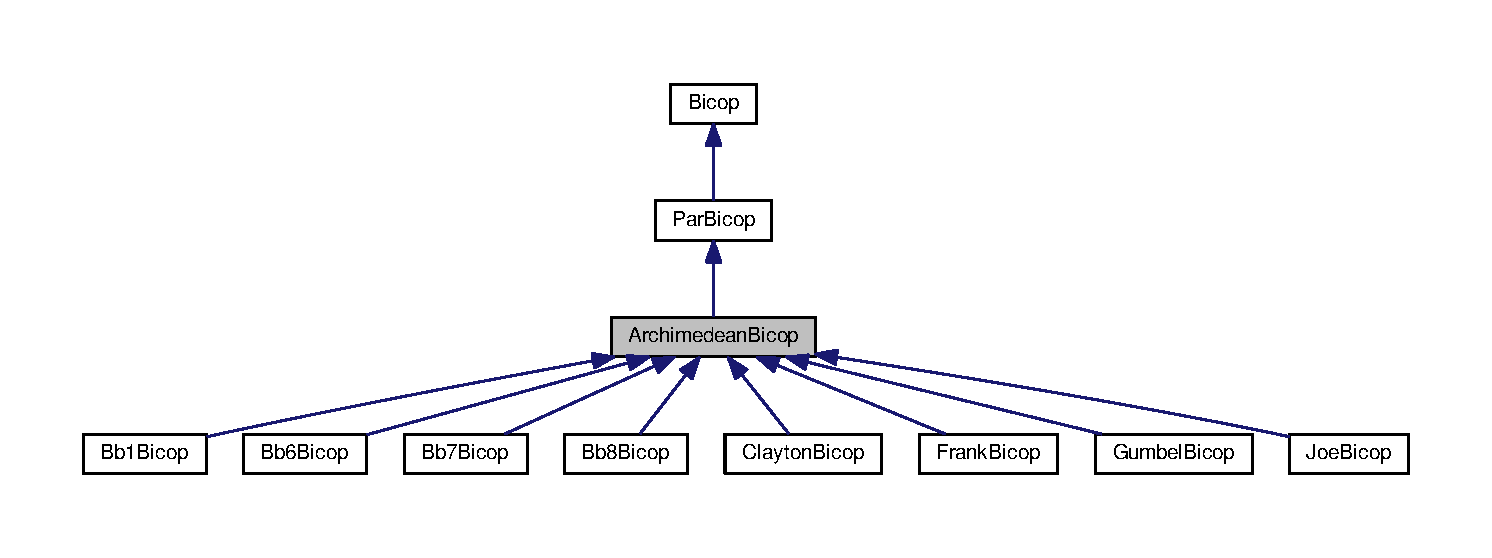
\includegraphics[width=350pt]{class_archimedean_bicop__inherit__graph}
\end{center}
\end{figure}


Collaboration diagram for Archimedean\+Bicop\+:\nopagebreak
\begin{figure}[H]
\begin{center}
\leavevmode
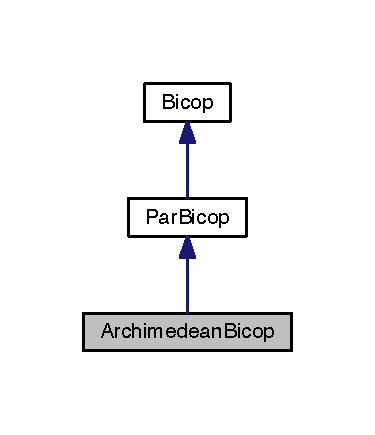
\includegraphics[width=176pt]{class_archimedean_bicop__coll__graph}
\end{center}
\end{figure}
\subsection*{Public Member Functions}
\begin{DoxyCompactItemize}
\item 
\hypertarget{class_archimedean_bicop_adee082ce9b2f7cc4a3408d67ed6b49f5}{Vec\+Xd {\bfseries pdf\+\_\+default} (const Mat\+Xd \&u)}\label{class_archimedean_bicop_adee082ce9b2f7cc4a3408d67ed6b49f5}

\item 
\hypertarget{class_archimedean_bicop_a912effaac24a1c94aa1e1d4b08819d75}{Vec\+Xd {\bfseries hfunc1\+\_\+default} (const Mat\+Xd \&u)}\label{class_archimedean_bicop_a912effaac24a1c94aa1e1d4b08819d75}

\item 
\hypertarget{class_archimedean_bicop_a1651e16c4534ca99cd58eaf8602b8525}{Vec\+Xd {\bfseries hfunc2\+\_\+default} (const Mat\+Xd \&u)}\label{class_archimedean_bicop_a1651e16c4534ca99cd58eaf8602b8525}

\item 
\hypertarget{class_archimedean_bicop_a5c5a8569bad4be9e92ccd4434305806b}{Vec\+Xd {\bfseries hinv1\+\_\+default} (const Mat\+Xd \&u)}\label{class_archimedean_bicop_a5c5a8569bad4be9e92ccd4434305806b}

\item 
\hypertarget{class_archimedean_bicop_a6bac4cee0e824719b107477a06caf19e}{Vec\+Xd {\bfseries hinv2\+\_\+default} (const Mat\+Xd \&u)}\label{class_archimedean_bicop_a6bac4cee0e824719b107477a06caf19e}

\item 
\hypertarget{class_archimedean_bicop_a9b79997308dc154a23808b84a863c563}{virtual Vec\+Xd {\bfseries generator} (const Vec\+Xd \&u)=0}\label{class_archimedean_bicop_a9b79997308dc154a23808b84a863c563}

\item 
\hypertarget{class_archimedean_bicop_af12082f1046554e0121b2c7d93148f13}{virtual Vec\+Xd {\bfseries generator\+\_\+inv} (const Vec\+Xd \&u)=0}\label{class_archimedean_bicop_af12082f1046554e0121b2c7d93148f13}

\item 
\hypertarget{class_archimedean_bicop_a9a18bbc021eb033c5b7d992d6d572b9b}{virtual Vec\+Xd {\bfseries generator\+\_\+derivative} (const Vec\+Xd \&u)=0}\label{class_archimedean_bicop_a9a18bbc021eb033c5b7d992d6d572b9b}

\item 
\hypertarget{class_archimedean_bicop_a16d7c2474e7e9bd16fa60a02550762ed}{virtual Vec\+Xd {\bfseries generator\+\_\+derivative2} (const Vec\+Xd \&u)=0}\label{class_archimedean_bicop_a16d7c2474e7e9bd16fa60a02550762ed}

\item 
\hypertarget{class_archimedean_bicop_ad9f6cd9ae6ca06f0d2edea2a52f195c9}{virtual Vec\+Xd {\bfseries hinv} (const Mat\+Xd \&u)=0}\label{class_archimedean_bicop_ad9f6cd9ae6ca06f0d2edea2a52f195c9}

\item 
\hypertarget{class_archimedean_bicop_afc56334b1c34406b5148386d9b7e5f43}{void \hyperlink{class_archimedean_bicop_afc56334b1c34406b5148386d9b7e5f43}{flip} ()}\label{class_archimedean_bicop_afc56334b1c34406b5148386d9b7e5f43}

\begin{DoxyCompactList}\small\item\em Adjust the copula to a flipping of arguments (u,v) -\/$>$ (v,u) \end{DoxyCompactList}\end{DoxyCompactItemize}
\subsection*{Additional Inherited Members}

\hypertarget{class_bicop}{}\section{Bicop Class Reference}
\label{class_bicop}\index{Bicop@{Bicop}}


{\ttfamily \#include $<$bicop\+\_\+class.\+hpp$>$}



Inheritance diagram for Bicop\+:\nopagebreak
\begin{figure}[H]
\begin{center}
\leavevmode
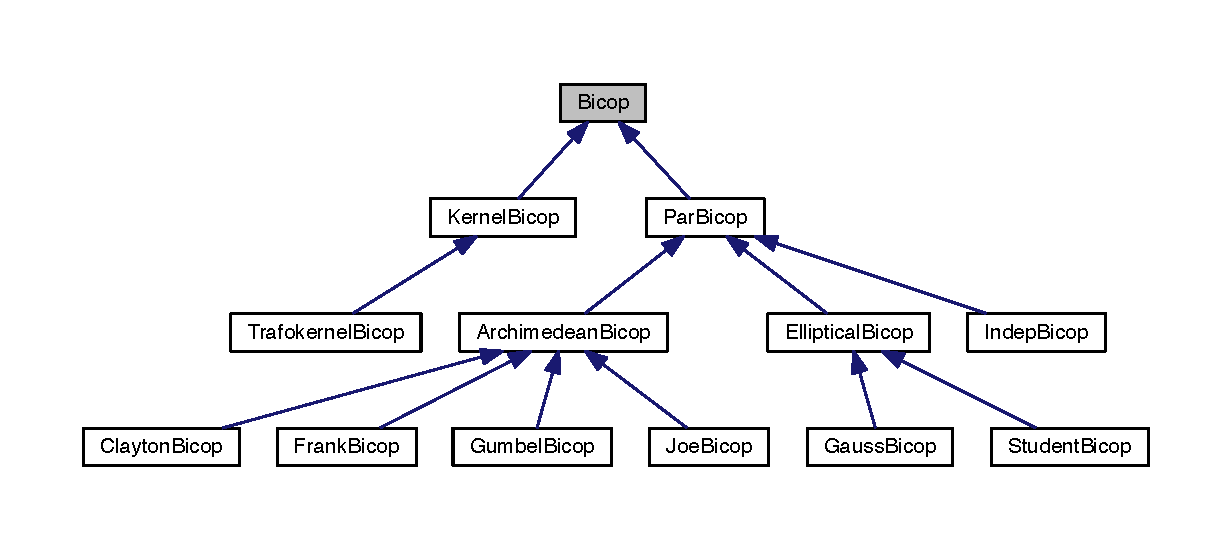
\includegraphics[width=350pt]{class_bicop__inherit__graph}
\end{center}
\end{figure}
\subsection*{Public Member Functions}
\begin{DoxyCompactItemize}
\item 
Vec\+Xd {\bfseries pdf} (const Mat\+Xd \&u)
\item 
Vec\+Xd {\bfseries hfunc1} (const Mat\+Xd \&u)
\item 
Vec\+Xd {\bfseries hfunc2} (const Mat\+Xd \&u)
\item 
Vec\+Xd {\bfseries hinv1} (const Mat\+Xd \&u)
\item 
Vec\+Xd {\bfseries hinv2} (const Mat\+Xd \&u)
\item 
Mat\+Xd \hyperlink{class_bicop_afa62d40a17e096cc0f7e769fb2a1285d}{simulate} (const int \&n)
\item 
virtual double \hyperlink{class_bicop_a21f37d9e51460c13be57e48c3d1e7ba4}{calculate\+\_\+npars} ()=0\hypertarget{class_bicop_a21f37d9e51460c13be57e48c3d1e7ba4}{}\label{class_bicop_a21f37d9e51460c13be57e48c3d1e7ba4}

\begin{DoxyCompactList}\small\item\em Get number of parameters. \end{DoxyCompactList}\item 
double \hyperlink{class_bicop_abe228ece449fb66996f91b0fcfed60d3}{calculate\+\_\+tau} ()\hypertarget{class_bicop_abe228ece449fb66996f91b0fcfed60d3}{}\label{class_bicop_abe228ece449fb66996f91b0fcfed60d3}

\begin{DoxyCompactList}\small\item\em Calculate the theoretical Kendall\textquotesingle{}s tau. \end{DoxyCompactList}\item 
virtual double {\bfseries parameters\+\_\+to\+\_\+tau} (const Vec\+Xd \&parameters)=0\hypertarget{class_bicop_aadd4f372b89a2389348893633ec238ba}{}\label{class_bicop_aadd4f372b89a2389348893633ec238ba}

\item 
Vec\+Xd \hyperlink{class_bicop_af20cc82a278f7c5a40dca399402caf10}{tau\+\_\+to\+\_\+parameters} (const double \&tau)\hypertarget{class_bicop_af20cc82a278f7c5a40dca399402caf10}{}\label{class_bicop_af20cc82a278f7c5a40dca399402caf10}

\begin{DoxyCompactList}\small\item\em Extract the copula parameter from Kendall\textquotesingle{}s tau whenever possible. \end{DoxyCompactList}\item 
virtual void \hyperlink{class_bicop_ac7d72dc620a2de66f6c1136329d1b4a3}{flip} ()=0\hypertarget{class_bicop_ac7d72dc620a2de66f6c1136329d1b4a3}{}\label{class_bicop_ac7d72dc620a2de66f6c1136329d1b4a3}

\begin{DoxyCompactList}\small\item\em Adjust the copula to a flipping of arguments (u,v) -\/$>$ (v,u) \end{DoxyCompactList}\end{DoxyCompactItemize}
{\bf }\par
\begin{DoxyCompactItemize}
\item 
virtual void \hyperlink{class_bicop_a0ff40d8054e11ed8aaa4956c7fd84e89}{fit} (const Mat\+Xd \&data, std\+::string method)=0
\item 
double {\bfseries loglik} (const Mat\+Xd \&u)\hypertarget{class_bicop_a994d28aa99b881425f012605aef3ae68}{}\label{class_bicop_a994d28aa99b881425f012605aef3ae68}

\item 
double {\bfseries aic} (const Mat\+Xd \&u)\hypertarget{class_bicop_adb4aecd877fc32cc857e2477d5bddf9b}{}\label{class_bicop_adb4aecd877fc32cc857e2477d5bddf9b}

\item 
double {\bfseries bic} (const Mat\+Xd \&u)\hypertarget{class_bicop_a68ee43f29c026aaf8157673c1ddf29b2}{}\label{class_bicop_a68ee43f29c026aaf8157673c1ddf29b2}

\end{DoxyCompactItemize}

{\bf }\par
\begin{DoxyCompactItemize}
\item 
int \hyperlink{class_bicop_a78a564f6e071e8dba7bcd93fdd1b05a4}{get\+\_\+family} () const 
\item 
int {\bfseries get\+\_\+rotation} () const \hypertarget{class_bicop_a0cf41f139c731d37841a411be5123155}{}\label{class_bicop_a0cf41f139c731d37841a411be5123155}

\item 
std\+::string {\bfseries get\+\_\+association\+\_\+direction} () const \hypertarget{class_bicop_a6758285bf2e354bbfbf8f8e0465567ba}{}\label{class_bicop_a6758285bf2e354bbfbf8f8e0465567ba}

\item 
Vec\+Xd {\bfseries get\+\_\+parameters} () const \hypertarget{class_bicop_a5ae1eb1665235ea822f0f62b69085047}{}\label{class_bicop_a5ae1eb1665235ea822f0f62b69085047}

\item 
Mat\+Xd {\bfseries get\+\_\+parameters\+\_\+bounds} () const \hypertarget{class_bicop_af3387cb6498e8b08c23d442a437ef6e0}{}\label{class_bicop_af3387cb6498e8b08c23d442a437ef6e0}

\item 
void {\bfseries set\+\_\+rotation} (const int \&rotation)\hypertarget{class_bicop_af5cded47298fa11fc0f997d7a873cf92}{}\label{class_bicop_af5cded47298fa11fc0f997d7a873cf92}

\item 
void {\bfseries set\+\_\+parameters} (const Vec\+Xd \&parameters)\hypertarget{class_bicop_a86d6d832e19d4e947fad68590e6f1b40}{}\label{class_bicop_a86d6d832e19d4e947fad68590e6f1b40}

\end{DoxyCompactItemize}

\subsection*{Static Public Member Functions}
\begin{DoxyCompactItemize}
\item 
static std\+::shared\+\_\+ptr$<$ \hyperlink{class_bicop}{Bicop} $>$ \hyperlink{class_bicop_acb60163725518f4ccfd7694272014686}{create} (const int \&family, const int \&rotation)
\item 
static std\+::shared\+\_\+ptr$<$ \hyperlink{class_bicop}{Bicop} $>$ \hyperlink{class_bicop_a4bfa38e69a96cc8a7c689e1161942e46}{create} (const int \&family, const Vec\+Xd \&parameters, const int \&rotation)
\item 
static std\+::shared\+\_\+ptr$<$ \hyperlink{class_bicop}{Bicop} $>$ \hyperlink{class_bicop_a6b1c154595bb17cd73f81cb4f563a776}{select} (const Mat\+Xd \&data, std\+::string selection\+\_\+criterion, std\+::vector$<$ int $>$ family\+\_\+set, bool use\+\_\+rotations, bool preselect\+\_\+families, std\+::string method)
\end{DoxyCompactItemize}
\subsection*{Protected Member Functions}
\begin{DoxyCompactItemize}
\item 
virtual Vec\+Xd {\bfseries pdf\+\_\+default} (const Mat\+Xd \&u)=0\hypertarget{class_bicop_a89e76fb74a9a4583cd74ce7bd72b5821}{}\label{class_bicop_a89e76fb74a9a4583cd74ce7bd72b5821}

\item 
virtual Vec\+Xd {\bfseries hfunc1\+\_\+default} (const Mat\+Xd \&u)=0\hypertarget{class_bicop_a60b997ec055f573034fc1736470ed7db}{}\label{class_bicop_a60b997ec055f573034fc1736470ed7db}

\item 
virtual Vec\+Xd {\bfseries hfunc2\+\_\+default} (const Mat\+Xd \&u)=0\hypertarget{class_bicop_afb7f326409f22b6b65e46f89dcf5ee1a}{}\label{class_bicop_afb7f326409f22b6b65e46f89dcf5ee1a}

\item 
virtual Vec\+Xd {\bfseries hinv1\+\_\+default} (const Mat\+Xd \&u)=0\hypertarget{class_bicop_a401bdcb4172c55b3d5f0c2a0db30ca43}{}\label{class_bicop_a401bdcb4172c55b3d5f0c2a0db30ca43}

\item 
virtual Vec\+Xd {\bfseries hinv2\+\_\+default} (const Mat\+Xd \&u)=0\hypertarget{class_bicop_a046b0fdc43eed27002f0b7c3bc9a9ddb}{}\label{class_bicop_a046b0fdc43eed27002f0b7c3bc9a9ddb}

\item 
Vec\+Xd \hyperlink{class_bicop_abd517becaa97834eac56b0d1a0c7a666}{hinv1\+\_\+num} (const Mat\+Xd \&u)
\item 
Vec\+Xd {\bfseries hinv2\+\_\+num} (const Mat\+Xd \&u)\hypertarget{class_bicop_a2b262e9e2adee0c215da47467f1dec45}{}\label{class_bicop_a2b262e9e2adee0c215da47467f1dec45}

\item 
Mat\+Xd \hyperlink{class_bicop_a48dc314b01b0c5b0adb307d27d4dd53e}{cut\+\_\+and\+\_\+rotate} (const Mat\+Xd \&u)
\item 
Mat\+Xd {\bfseries swap\+\_\+cols} (const Mat\+Xd \&u)\hypertarget{class_bicop_a96e06c8996e378d56d9e87ff4d1a24ac}{}\label{class_bicop_a96e06c8996e378d56d9e87ff4d1a24ac}

\end{DoxyCompactItemize}
\subsection*{Protected Attributes}
\begin{DoxyCompactItemize}
\item 
int {\bfseries family\+\_\+}\hypertarget{class_bicop_a3d546f9b8c6507002cae18b9fdcb4544}{}\label{class_bicop_a3d546f9b8c6507002cae18b9fdcb4544}

\item 
std\+::string {\bfseries family\+\_\+name\+\_\+}\hypertarget{class_bicop_ae87af8dcf838aa9342baf814f1a9c0c7}{}\label{class_bicop_ae87af8dcf838aa9342baf814f1a9c0c7}

\item 
int {\bfseries rotation\+\_\+}\hypertarget{class_bicop_a606833e2ea1d17a318dd20d67d01b40a}{}\label{class_bicop_a606833e2ea1d17a318dd20d67d01b40a}

\item 
std\+::string {\bfseries association\+\_\+direction\+\_\+}\hypertarget{class_bicop_a407914da267317da3f588632e4b95aa3}{}\label{class_bicop_a407914da267317da3f588632e4b95aa3}

\item 
Vec\+Xd {\bfseries parameters\+\_\+}\hypertarget{class_bicop_ade78fec591e6699a808b63104709b23a}{}\label{class_bicop_ade78fec591e6699a808b63104709b23a}

\item 
Mat\+Xd {\bfseries parameters\+\_\+bounds\+\_\+}\hypertarget{class_bicop_aa1253f11c251ea6d9f4020317e4346ab}{}\label{class_bicop_aa1253f11c251ea6d9f4020317e4346ab}

\end{DoxyCompactItemize}


\subsection{Detailed Description}
A class for bivariate copulas

The \hyperlink{class_bicop}{Bicop} class is abstract, you cannot create an instance of this class, but only of the derived classes. 

\subsection{Member Function Documentation}
\index{Bicop@{Bicop}!create@{create}}
\index{create@{create}!Bicop@{Bicop}}
\subsubsection[{\texorpdfstring{create(const int \&family, const int \&rotation)}{create(const int &family, const int &rotation)}}]{\setlength{\rightskip}{0pt plus 5cm}Bicop\+Ptr Bicop\+::create (
\begin{DoxyParamCaption}
\item[{const int \&}]{family, }
\item[{const int \&}]{rotation}
\end{DoxyParamCaption}
)\hspace{0.3cm}{\ttfamily [static]}}\hypertarget{class_bicop_acb60163725518f4ccfd7694272014686}{}\label{class_bicop_acb60163725518f4ccfd7694272014686}
Create a bivariate copula using the default contructor


\begin{DoxyParams}{Parameters}
{\em family} & the copula family. \\
\hline
{\em rotation} & the rotation type. \\
\hline
\end{DoxyParams}
\begin{DoxyReturn}{Returns}
A pointer to an object that inherits from {\ttfamily \hyperlink{class_bicop}{Bicop}}. 
\end{DoxyReturn}
\index{Bicop@{Bicop}!create@{create}}
\index{create@{create}!Bicop@{Bicop}}
\subsubsection[{\texorpdfstring{create(const int \&family, const Vec\+Xd \&parameters, const int \&rotation)}{create(const int &family, const VecXd &parameters, const int &rotation)}}]{\setlength{\rightskip}{0pt plus 5cm}Bicop\+Ptr Bicop\+::create (
\begin{DoxyParamCaption}
\item[{const int \&}]{family, }
\item[{const Vec\+Xd \&}]{parameters, }
\item[{const int \&}]{rotation}
\end{DoxyParamCaption}
)\hspace{0.3cm}{\ttfamily [static]}}\hypertarget{class_bicop_a4bfa38e69a96cc8a7c689e1161942e46}{}\label{class_bicop_a4bfa38e69a96cc8a7c689e1161942e46}
Create a bivariate copula with a specified parameters vector


\begin{DoxyParams}{Parameters}
{\em family} & the copula family. \\
\hline
{\em par} & the copula parameters (must be compatible with family). \\
\hline
{\em rotation} & the rotation type. \\
\hline
\end{DoxyParams}
\begin{DoxyReturn}{Returns}
A pointer to an object that inherits from {\ttfamily \hyperlink{class_bicop}{Bicop}}. 
\end{DoxyReturn}
\index{Bicop@{Bicop}!cut\+\_\+and\+\_\+rotate@{cut\+\_\+and\+\_\+rotate}}
\index{cut\+\_\+and\+\_\+rotate@{cut\+\_\+and\+\_\+rotate}!Bicop@{Bicop}}
\subsubsection[{\texorpdfstring{cut\+\_\+and\+\_\+rotate(const Mat\+Xd \&u)}{cut_and_rotate(const MatXd &u)}}]{\setlength{\rightskip}{0pt plus 5cm}Mat\+Xd Bicop\+::cut\+\_\+and\+\_\+rotate (
\begin{DoxyParamCaption}
\item[{const Mat\+Xd \&}]{u}
\end{DoxyParamCaption}
)\hspace{0.3cm}{\ttfamily [protected]}}\hypertarget{class_bicop_a48dc314b01b0c5b0adb307d27d4dd53e}{}\label{class_bicop_a48dc314b01b0c5b0adb307d27d4dd53e}
Data manipulations for rotated families


\begin{DoxyParams}{Parameters}
{\em u} & $m \times 2$ matrix of evaluation points. \\
\hline
\end{DoxyParams}
\index{Bicop@{Bicop}!fit@{fit}}
\index{fit@{fit}!Bicop@{Bicop}}
\subsubsection[{\texorpdfstring{fit(const Mat\+Xd \&data, std\+::string method)=0}{fit(const MatXd &data, std::string method)=0}}]{\setlength{\rightskip}{0pt plus 5cm}virtual void Bicop\+::fit (
\begin{DoxyParamCaption}
\item[{const Mat\+Xd \&}]{data, }
\item[{std\+::string}]{method}
\end{DoxyParamCaption}
)\hspace{0.3cm}{\ttfamily [pure virtual]}}\hypertarget{class_bicop_a0ff40d8054e11ed8aaa4956c7fd84e89}{}\label{class_bicop_a0ff40d8054e11ed8aaa4956c7fd84e89}
fitstats Fit methods and statistics


\begin{DoxyParams}{Parameters}
{\em u} & $m \times 2$ matrix of observations. \\
\hline
\end{DoxyParams}


Implemented in \hyperlink{class_par_bicop_aeab5e7031792bebc04a401a8f135d3a0}{Par\+Bicop}, and \hyperlink{class_trafokernel_bicop_ae5da9284cd058b02878614059d8ce078}{Trafokernel\+Bicop}.

\index{Bicop@{Bicop}!get\+\_\+family@{get\+\_\+family}}
\index{get\+\_\+family@{get\+\_\+family}!Bicop@{Bicop}}
\subsubsection[{\texorpdfstring{get\+\_\+family() const }{get_family() const }}]{\setlength{\rightskip}{0pt plus 5cm}int Bicop\+::get\+\_\+family (
\begin{DoxyParamCaption}
{}
\end{DoxyParamCaption}
) const\hspace{0.3cm}{\ttfamily [inline]}}\hypertarget{class_bicop_a78a564f6e071e8dba7bcd93fdd1b05a4}{}\label{class_bicop_a78a564f6e071e8dba7bcd93fdd1b05a4}
Getters and setters. \index{Bicop@{Bicop}!hinv1\+\_\+num@{hinv1\+\_\+num}}
\index{hinv1\+\_\+num@{hinv1\+\_\+num}!Bicop@{Bicop}}
\subsubsection[{\texorpdfstring{hinv1\+\_\+num(const Mat\+Xd \&u)}{hinv1_num(const MatXd &u)}}]{\setlength{\rightskip}{0pt plus 5cm}Vec\+Xd Bicop\+::hinv1\+\_\+num (
\begin{DoxyParamCaption}
\item[{const Mat\+Xd \&}]{u}
\end{DoxyParamCaption}
)\hspace{0.3cm}{\ttfamily [protected]}}\hypertarget{class_bicop_abd517becaa97834eac56b0d1a0c7a666}{}\label{class_bicop_abd517becaa97834eac56b0d1a0c7a666}
Numerical inversion of h-\/functions

These are generic functions to invert the hfunctions numerically. They can be used in derived classes to define {\ttfamily hinv1} and {\ttfamily hinv2}.


\begin{DoxyParams}{Parameters}
{\em u} & $m \times 2$ matrix of evaluation points. \\
\hline
\end{DoxyParams}
\index{Bicop@{Bicop}!select@{select}}
\index{select@{select}!Bicop@{Bicop}}
\subsubsection[{\texorpdfstring{select(const Mat\+Xd \&data, std\+::string selection\+\_\+criterion, std\+::vector$<$ int $>$ family\+\_\+set, bool use\+\_\+rotations, bool preselect\+\_\+families, std\+::string method)}{select(const MatXd &data, std::string selection_criterion, std::vector< int > family_set, bool use_rotations, bool preselect_families, std::string method)}}]{\setlength{\rightskip}{0pt plus 5cm}Bicop\+Ptr Bicop\+::select (
\begin{DoxyParamCaption}
\item[{const Mat\+Xd \&}]{data, }
\item[{std\+::string}]{selection\+\_\+criterion, }
\item[{std\+::vector$<$ int $>$}]{family\+\_\+set, }
\item[{bool}]{use\+\_\+rotations, }
\item[{bool}]{preselect\+\_\+families, }
\item[{std\+::string}]{method}
\end{DoxyParamCaption}
)\hspace{0.3cm}{\ttfamily [static]}}\hypertarget{class_bicop_a6b1c154595bb17cd73f81cb4f563a776}{}\label{class_bicop_a6b1c154595bb17cd73f81cb4f563a776}
Select a bivariate copula


\begin{DoxyParams}{Parameters}
{\em data} & the data to fit the bivariate copula. \\
\hline
{\em selection\+\_\+criterion} & the selection criterion (\char`\"{}aic\char`\"{} or \char`\"{}bic\char`\"{}). \\
\hline
{\em family\+\_\+set} & the set of copula families to consider (if empty, then all families are included). \\
\hline
{\em use\+\_\+rotations} & whether rotations in the familyset are included. \\
\hline
{\em preselect\+\_\+families} & whether to exclude families before fitting based on symmetry properties of the data. \\
\hline
{\em method} & indicates the estimation method\+: either maximum likelihood estimation (method = \char`\"{}mle\char`\"{}) or inversion of Kendall\textquotesingle{}s tau (method = \char`\"{}itau\char`\"{}). When method = \char`\"{}itau\char`\"{} is used with families having more than one parameter, the main dependence parameter is found by inverting the Kendall\textquotesingle{}s tau and the remainders by a profile likelihood optimization. \\
\hline
\end{DoxyParams}
\begin{DoxyReturn}{Returns}
A pointer to an object that inherits from {\ttfamily \hyperlink{class_bicop}{Bicop}}. 
\end{DoxyReturn}
\index{Bicop@{Bicop}!simulate@{simulate}}
\index{simulate@{simulate}!Bicop@{Bicop}}
\subsubsection[{\texorpdfstring{simulate(const int \&n)}{simulate(const int &n)}}]{\setlength{\rightskip}{0pt plus 5cm}Mat\+Xd Bicop\+::simulate (
\begin{DoxyParamCaption}
\item[{const int \&}]{n}
\end{DoxyParamCaption}
)}\hypertarget{class_bicop_afa62d40a17e096cc0f7e769fb2a1285d}{}\label{class_bicop_afa62d40a17e096cc0f7e769fb2a1285d}
Simulate from a bivariate copula


\begin{DoxyParams}{Parameters}
{\em n} & number of observations. \\
\hline
\end{DoxyParams}


The documentation for this class was generated from the following files\+:\begin{DoxyCompactItemize}
\item 
/home/n5/dev/cpp/vinecopulib/include/bicop\+\_\+class.\+hpp\item 
/home/n5/dev/cpp/vinecopulib/src/bicop\+\_\+class.\+cpp\end{DoxyCompactItemize}

\hypertarget{class_clayton_bicop}{\section{Clayton\+Bicop Class Reference}
\label{class_clayton_bicop}\index{Clayton\+Bicop@{Clayton\+Bicop}}
}


Inheritance diagram for Clayton\+Bicop\+:
\nopagebreak
\begin{figure}[H]
\begin{center}
\leavevmode
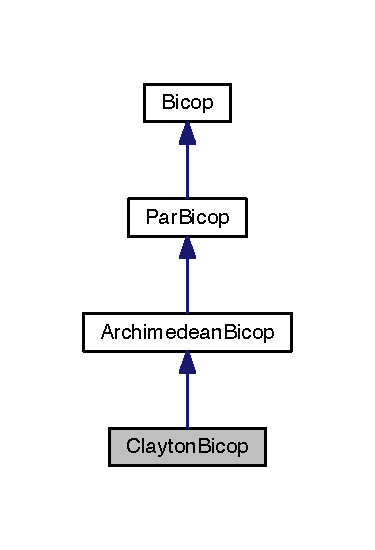
\includegraphics[width=176pt]{class_clayton_bicop__inherit__graph}
\end{center}
\end{figure}


Collaboration diagram for Clayton\+Bicop\+:
\nopagebreak
\begin{figure}[H]
\begin{center}
\leavevmode
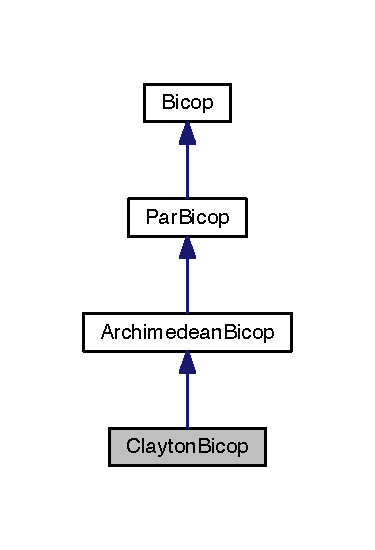
\includegraphics[width=176pt]{class_clayton_bicop__coll__graph}
\end{center}
\end{figure}
\subsection*{Public Member Functions}
\begin{DoxyCompactItemize}
\item 
\hypertarget{class_clayton_bicop_a6e3b29b40f19424886c0f4b673977515}{{\bfseries Clayton\+Bicop} (double theta)}\label{class_clayton_bicop_a6e3b29b40f19424886c0f4b673977515}

\item 
\hypertarget{class_clayton_bicop_a225581e47b5c1047091be8cc070fcdae}{{\bfseries Clayton\+Bicop} (double theta, int rotation)}\label{class_clayton_bicop_a225581e47b5c1047091be8cc070fcdae}

\item 
\hypertarget{class_clayton_bicop_a9763aabca37806261b8ecd6c46f4cf95}{Vec\+Xd {\bfseries generator} (const Vec\+Xd \&u)}\label{class_clayton_bicop_a9763aabca37806261b8ecd6c46f4cf95}

\item 
\hypertarget{class_clayton_bicop_a295caa6493575640a96201414dbf398f}{Vec\+Xd {\bfseries generator\+\_\+inv} (const Vec\+Xd \&u)}\label{class_clayton_bicop_a295caa6493575640a96201414dbf398f}

\item 
\hypertarget{class_clayton_bicop_ab009f6aa6036ad92d83a3d185e6234d8}{Vec\+Xd {\bfseries generator\+\_\+derivative} (const Vec\+Xd \&u)}\label{class_clayton_bicop_ab009f6aa6036ad92d83a3d185e6234d8}

\item 
\hypertarget{class_clayton_bicop_af24c631fbf12bcf3f52724fcf926cfef}{Vec\+Xd {\bfseries generator\+\_\+derivative2} (const Vec\+Xd \&u)}\label{class_clayton_bicop_af24c631fbf12bcf3f52724fcf926cfef}

\item 
\hypertarget{class_clayton_bicop_a087f50080b50c8ae0c545b7b182ba983}{Mat\+Xd {\bfseries get\+\_\+bounds\+\_\+standard} ()}\label{class_clayton_bicop_a087f50080b50c8ae0c545b7b182ba983}

\item 
\hypertarget{class_clayton_bicop_a3de44e26cffcac6d7e2511cc1ad56b04}{Vec\+Xd {\bfseries hinv} (const Mat\+Xd \&u)}\label{class_clayton_bicop_a3de44e26cffcac6d7e2511cc1ad56b04}

\item 
\hypertarget{class_clayton_bicop_a86b6e4ba35a2563b826b7811e7de3b47}{double {\bfseries tau\+\_\+to\+\_\+par} (double \&tau)}\label{class_clayton_bicop_a86b6e4ba35a2563b826b7811e7de3b47}

\item 
\hypertarget{class_clayton_bicop_a874e76cdb70e2e6ad2ee27596f3bfdc2}{double {\bfseries par\+\_\+to\+\_\+tau} (double \&par)}\label{class_clayton_bicop_a874e76cdb70e2e6ad2ee27596f3bfdc2}

\end{DoxyCompactItemize}
\subsection*{Additional Inherited Members}


The documentation for this class was generated from the following files\+:\begin{DoxyCompactItemize}
\item 
/home/data/uni/\+Promotion/\+Cpp/vinecoplib/src/common/include/bicop\+\_\+clayton.\+hpp\item 
/home/data/uni/\+Promotion/\+Cpp/vinecoplib/src/common/bicop\+\_\+clayton.\+cpp\end{DoxyCompactItemize}

\hypertarget{class_elliptical_bicop}{\section{Elliptical\+Bicop Class Reference}
\label{class_elliptical_bicop}\index{Elliptical\+Bicop@{Elliptical\+Bicop}}
}


Inheritance diagram for Elliptical\+Bicop\+:\nopagebreak
\begin{figure}[H]
\begin{center}
\leavevmode
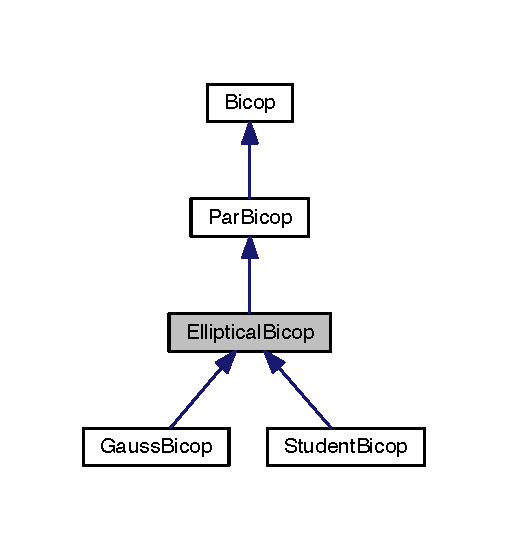
\includegraphics[width=243pt]{class_elliptical_bicop__inherit__graph}
\end{center}
\end{figure}


Collaboration diagram for Elliptical\+Bicop\+:\nopagebreak
\begin{figure}[H]
\begin{center}
\leavevmode
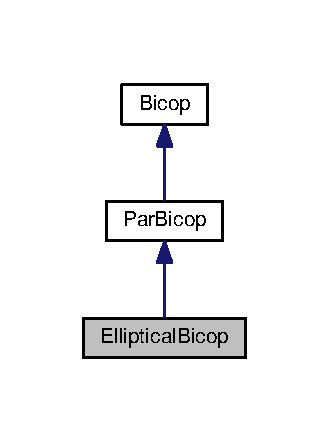
\includegraphics[width=158pt]{class_elliptical_bicop__coll__graph}
\end{center}
\end{figure}
\subsection*{Public Member Functions}
\begin{DoxyCompactItemize}
\item 
\hypertarget{class_elliptical_bicop_a9d859278685c80465d09dc8fe05b7d3d}{virtual Vec\+Xd {\bfseries pdf\+\_\+default} (const Mat\+Xd \&u)=0}\label{class_elliptical_bicop_a9d859278685c80465d09dc8fe05b7d3d}

\item 
\hypertarget{class_elliptical_bicop_ae4e47a0b9373b0f103b28fbacdaa58b8}{virtual Vec\+Xd {\bfseries hfunc1\+\_\+default} (const Mat\+Xd \&u)=0}\label{class_elliptical_bicop_ae4e47a0b9373b0f103b28fbacdaa58b8}

\item 
\hypertarget{class_elliptical_bicop_a18f5fa85bd6ed14d56e0b269c091ac3b}{Vec\+Xd {\bfseries hfunc2\+\_\+default} (const Mat\+Xd \&u)}\label{class_elliptical_bicop_a18f5fa85bd6ed14d56e0b269c091ac3b}

\item 
\hypertarget{class_elliptical_bicop_aa2a3700bc5dd43aade311985f96077e0}{virtual Vec\+Xd {\bfseries hinv1\+\_\+default} (const Mat\+Xd \&u)=0}\label{class_elliptical_bicop_aa2a3700bc5dd43aade311985f96077e0}

\item 
\hypertarget{class_elliptical_bicop_ac94477889cbd73c30eb7010001e9fec8}{Vec\+Xd {\bfseries hinv2\+\_\+default} (const Mat\+Xd \&u)}\label{class_elliptical_bicop_ac94477889cbd73c30eb7010001e9fec8}

\item 
\hypertarget{class_elliptical_bicop_a4a478ff32dddf4561c8d97041b943e1f}{Vec\+Xd {\bfseries tau\+\_\+to\+\_\+parameters} (const double \&tau)}\label{class_elliptical_bicop_a4a478ff32dddf4561c8d97041b943e1f}

\item 
\hypertarget{class_elliptical_bicop_a45f034c75af02d9b20b4af5c16754e5a}{double {\bfseries parameters\+\_\+to\+\_\+tau} (const Vec\+Xd \&parameters)}\label{class_elliptical_bicop_a45f034c75af02d9b20b4af5c16754e5a}

\item 
\hypertarget{class_elliptical_bicop_a176f55b005e74efe21abd01651ea8967}{void \hyperlink{class_elliptical_bicop_a176f55b005e74efe21abd01651ea8967}{flip} ()}\label{class_elliptical_bicop_a176f55b005e74efe21abd01651ea8967}

\begin{DoxyCompactList}\small\item\em Adjust the copula to a flipping of arguments (u,v) -\/$>$ (v,u) \end{DoxyCompactList}\end{DoxyCompactItemize}
\subsection*{Additional Inherited Members}

\hypertarget{class_frank_bicop}{}\section{Frank\+Bicop Class Reference}
\label{class_frank_bicop}\index{Frank\+Bicop@{Frank\+Bicop}}


Inheritance diagram for Frank\+Bicop\+:
\nopagebreak
\begin{figure}[H]
\begin{center}
\leavevmode
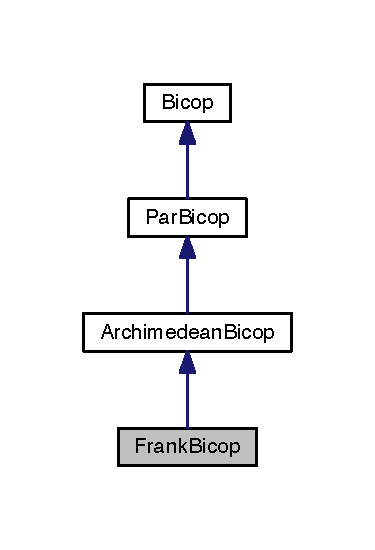
\includegraphics[width=180pt]{class_frank_bicop__inherit__graph}
\end{center}
\end{figure}


Collaboration diagram for Frank\+Bicop\+:
\nopagebreak
\begin{figure}[H]
\begin{center}
\leavevmode
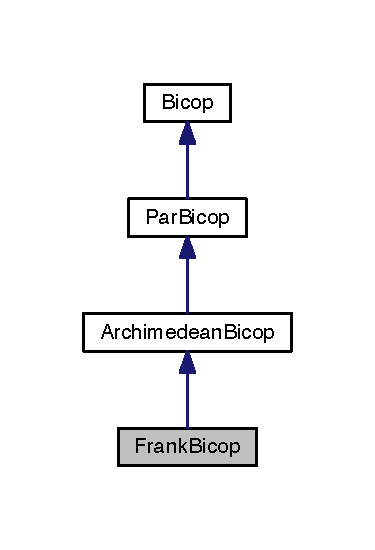
\includegraphics[width=180pt]{class_frank_bicop__coll__graph}
\end{center}
\end{figure}
\subsection*{Public Member Functions}
\begin{DoxyCompactItemize}
\item 
\mbox{\Hypertarget{class_frank_bicop_ae019221e15eba598f29d9120ac6d1f5c}\label{class_frank_bicop_ae019221e15eba598f29d9120ac6d1f5c}} 
{\bfseries Frank\+Bicop} (const Vec\+Xd \&parameters)
\item 
\mbox{\Hypertarget{class_frank_bicop_af789907cefc0049b2ce6ea4596195d48}\label{class_frank_bicop_af789907cefc0049b2ce6ea4596195d48}} 
{\bfseries Frank\+Bicop} (const Vec\+Xd \&parameters, const int \&rotation)
\item 
\mbox{\Hypertarget{class_frank_bicop_aac20b71ec67ea5067c5342c085a0e306}\label{class_frank_bicop_aac20b71ec67ea5067c5342c085a0e306}} 
Vec\+Xd {\bfseries generator} (const Vec\+Xd \&u)
\item 
\mbox{\Hypertarget{class_frank_bicop_a3e433ca2c858e95c11896d2d6a445648}\label{class_frank_bicop_a3e433ca2c858e95c11896d2d6a445648}} 
Vec\+Xd {\bfseries generator\+\_\+inv} (const Vec\+Xd \&u)
\item 
\mbox{\Hypertarget{class_frank_bicop_a19d2a80d449caa48d75690be81c2db02}\label{class_frank_bicop_a19d2a80d449caa48d75690be81c2db02}} 
Vec\+Xd {\bfseries generator\+\_\+derivative} (const Vec\+Xd \&u)
\item 
\mbox{\Hypertarget{class_frank_bicop_a07d9488138a598fa9aa770da2153f269}\label{class_frank_bicop_a07d9488138a598fa9aa770da2153f269}} 
Vec\+Xd {\bfseries generator\+\_\+derivative2} (const Vec\+Xd \&u)
\item 
\mbox{\Hypertarget{class_frank_bicop_ab755de64fbdf692303b4d6436bb41583}\label{class_frank_bicop_ab755de64fbdf692303b4d6436bb41583}} 
Vec\+Xd {\bfseries hinv} (const Mat\+Xd \&u)
\item 
\mbox{\Hypertarget{class_frank_bicop_ad4c350e726aa9ca7682d77c3e4e6ed3c}\label{class_frank_bicop_ad4c350e726aa9ca7682d77c3e4e6ed3c}} 
Vec\+Xd {\bfseries tau\+\_\+to\+\_\+parameters} (const double \&tau)
\item 
\mbox{\Hypertarget{class_frank_bicop_a59f4a4bbe5eb724d18091c2cd379e268}\label{class_frank_bicop_a59f4a4bbe5eb724d18091c2cd379e268}} 
double {\bfseries parameters\+\_\+to\+\_\+tau} (const Vec\+Xd \&par)
\end{DoxyCompactItemize}
\subsection*{Additional Inherited Members}


The documentation for this class was generated from the following files\+:\begin{DoxyCompactItemize}
\item 
/\+Users/tvatter/\+Dropbox/vinecoplib/vinecopulib/include/bicop\+\_\+frank.\+hpp\item 
/\+Users/tvatter/\+Dropbox/vinecoplib/vinecopulib/src/bicop\+\_\+frank.\+cpp\end{DoxyCompactItemize}

\hypertarget{class_gumbel_bicop}{\section{Gumbel\+Bicop Class Reference}
\label{class_gumbel_bicop}\index{Gumbel\+Bicop@{Gumbel\+Bicop}}
}


Inheritance diagram for Gumbel\+Bicop\+:
\nopagebreak
\begin{figure}[H]
\begin{center}
\leavevmode
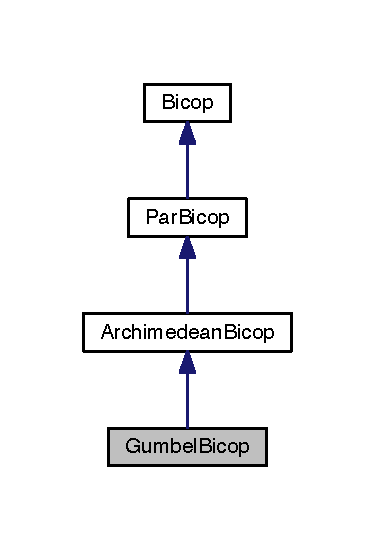
\includegraphics[width=176pt]{class_gumbel_bicop__inherit__graph}
\end{center}
\end{figure}


Collaboration diagram for Gumbel\+Bicop\+:
\nopagebreak
\begin{figure}[H]
\begin{center}
\leavevmode
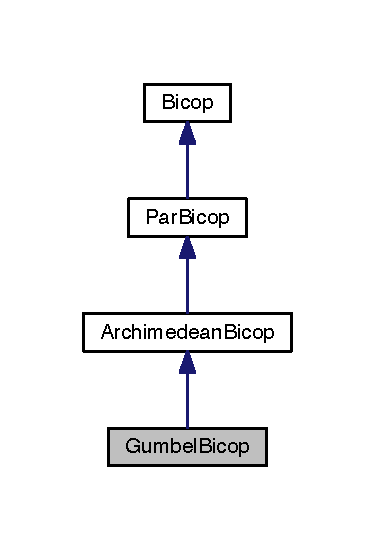
\includegraphics[width=176pt]{class_gumbel_bicop__coll__graph}
\end{center}
\end{figure}
\subsection*{Public Member Functions}
\begin{DoxyCompactItemize}
\item 
\hypertarget{class_gumbel_bicop_ab600aa2b30842d53add614f9c6617a4b}{{\bfseries Gumbel\+Bicop} (double theta)}\label{class_gumbel_bicop_ab600aa2b30842d53add614f9c6617a4b}

\item 
\hypertarget{class_gumbel_bicop_ae7f587608099dffb95e189609353e38a}{{\bfseries Gumbel\+Bicop} (double theta, int rotation)}\label{class_gumbel_bicop_ae7f587608099dffb95e189609353e38a}

\item 
\hypertarget{class_gumbel_bicop_a7462d2e917ed8f9c7c768bc763062000}{Vec\+Xd {\bfseries generator} (const Vec\+Xd \&u)}\label{class_gumbel_bicop_a7462d2e917ed8f9c7c768bc763062000}

\item 
\hypertarget{class_gumbel_bicop_a1aac5fc1926ebb1a7a5477fea8eafc4e}{Vec\+Xd {\bfseries generator\+\_\+inv} (const Vec\+Xd \&u)}\label{class_gumbel_bicop_a1aac5fc1926ebb1a7a5477fea8eafc4e}

\item 
\hypertarget{class_gumbel_bicop_a04ad137cdb969fdcb38141dd55cc08ca}{Vec\+Xd {\bfseries generator\+\_\+derivative} (const Vec\+Xd \&u)}\label{class_gumbel_bicop_a04ad137cdb969fdcb38141dd55cc08ca}

\item 
\hypertarget{class_gumbel_bicop_ab86b728ad0f0db50711e25defc39a1ad}{Vec\+Xd {\bfseries generator\+\_\+derivative2} (const Vec\+Xd \&u)}\label{class_gumbel_bicop_ab86b728ad0f0db50711e25defc39a1ad}

\item 
\hypertarget{class_gumbel_bicop_a33500ea02a83efb50cf1d5e6f32b928a}{Vec\+Xd {\bfseries hinv} (const Mat\+Xd \&u)}\label{class_gumbel_bicop_a33500ea02a83efb50cf1d5e6f32b928a}

\item 
\hypertarget{class_gumbel_bicop_ab1c5ed2bd052ff2f8a4f544cc213d62c}{double {\bfseries tau\+\_\+to\+\_\+par} (double \&tau)}\label{class_gumbel_bicop_ab1c5ed2bd052ff2f8a4f544cc213d62c}

\item 
\hypertarget{class_gumbel_bicop_a6a0b1e1a8dcf0f7d297f222ad3637337}{double {\bfseries par\+\_\+to\+\_\+tau} (double \&par)}\label{class_gumbel_bicop_a6a0b1e1a8dcf0f7d297f222ad3637337}

\item 
\hypertarget{class_gumbel_bicop_a05d34b9099cbb0a759604f2ad4b78d49}{Mat\+Xd {\bfseries get\+\_\+bounds\+\_\+standard} ()}\label{class_gumbel_bicop_a05d34b9099cbb0a759604f2ad4b78d49}

\end{DoxyCompactItemize}
\subsection*{Additional Inherited Members}


The documentation for this class was generated from the following files\+:\begin{DoxyCompactItemize}
\item 
/home/data/uni/\+Promotion/\+Cpp/vinecoplib/src/common/include/bicop\+\_\+gumbel.\+hpp\item 
/home/data/uni/\+Promotion/\+Cpp/vinecoplib/src/common/bicop\+\_\+gumbel.\+cpp\end{DoxyCompactItemize}

\hypertarget{class_indep_bicop}{}\section{Indep\+Bicop Class Reference}
\label{class_indep_bicop}\index{Indep\+Bicop@{Indep\+Bicop}}


Inheritance diagram for Indep\+Bicop\+:\nopagebreak
\begin{figure}[H]
\begin{center}
\leavevmode
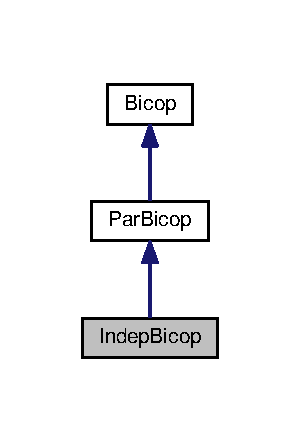
\includegraphics[width=145pt]{class_indep_bicop__inherit__graph}
\end{center}
\end{figure}


Collaboration diagram for Indep\+Bicop\+:\nopagebreak
\begin{figure}[H]
\begin{center}
\leavevmode
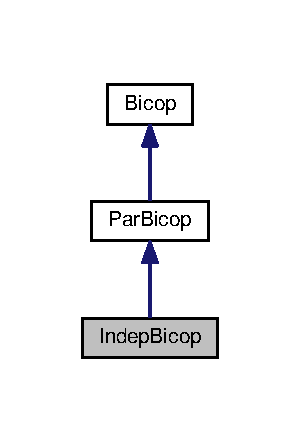
\includegraphics[width=145pt]{class_indep_bicop__coll__graph}
\end{center}
\end{figure}
\subsection*{Public Member Functions}
\begin{DoxyCompactItemize}
\item 
{\bfseries Indep\+Bicop} (const Vec\+Xd \&parameters)\hypertarget{class_indep_bicop_ab9f48d3291ac99c34e33c2f29b133e5d}{}\label{class_indep_bicop_ab9f48d3291ac99c34e33c2f29b133e5d}

\item 
{\bfseries Indep\+Bicop} (const Vec\+Xd \&parameters, const int \&rotation)\hypertarget{class_indep_bicop_ad7ead44250e4f421ec491b2d2a7eb030}{}\label{class_indep_bicop_ad7ead44250e4f421ec491b2d2a7eb030}

\item 
Vec\+Xd {\bfseries pdf\+\_\+default} (const Mat\+Xd \&u)\hypertarget{class_indep_bicop_a533aeb27876d38d9836929a71b9bb223}{}\label{class_indep_bicop_a533aeb27876d38d9836929a71b9bb223}

\item 
Vec\+Xd {\bfseries hfunc1\+\_\+default} (const Mat\+Xd \&u)\hypertarget{class_indep_bicop_abac716dd22bc020d073d50dfc552c00e}{}\label{class_indep_bicop_abac716dd22bc020d073d50dfc552c00e}

\item 
Vec\+Xd {\bfseries hfunc2\+\_\+default} (const Mat\+Xd \&u)\hypertarget{class_indep_bicop_ae054353b15c15d68a02b36a804e54dfa}{}\label{class_indep_bicop_ae054353b15c15d68a02b36a804e54dfa}

\item 
Vec\+Xd {\bfseries hinv1\+\_\+default} (const Mat\+Xd \&u)\hypertarget{class_indep_bicop_a61e64923f5b5a142d093c5b706893b93}{}\label{class_indep_bicop_a61e64923f5b5a142d093c5b706893b93}

\item 
Vec\+Xd {\bfseries hinv2\+\_\+default} (const Mat\+Xd \&u)\hypertarget{class_indep_bicop_a426311d78e6142d6f57e5a09080f9239}{}\label{class_indep_bicop_a426311d78e6142d6f57e5a09080f9239}

\item 
Vec\+Xd {\bfseries tau\+\_\+to\+\_\+parameters} (const double \&)\hypertarget{class_indep_bicop_ae2bcd4c9c3fadb947cce3d1915ca6f57}{}\label{class_indep_bicop_ae2bcd4c9c3fadb947cce3d1915ca6f57}

\item 
double {\bfseries parameters\+\_\+to\+\_\+tau} (const Vec\+Xd \&)\hypertarget{class_indep_bicop_a1f9a8f4bf6d0fc6a053ded53eb35015a}{}\label{class_indep_bicop_a1f9a8f4bf6d0fc6a053ded53eb35015a}

\item 
void \hyperlink{class_indep_bicop_ab6e5a7670b984d685241b6c998ff3381}{flip} ()\hypertarget{class_indep_bicop_ab6e5a7670b984d685241b6c998ff3381}{}\label{class_indep_bicop_ab6e5a7670b984d685241b6c998ff3381}

\begin{DoxyCompactList}\small\item\em Adjust the copula to a flipping of arguments (u,v) -\/$>$ (v,u) \end{DoxyCompactList}\end{DoxyCompactItemize}
\subsection*{Additional Inherited Members}


The documentation for this class was generated from the following files\+:\begin{DoxyCompactItemize}
\item 
/home/n5/dev/cpp/vinecopulib/include/bicop\+\_\+indep.\+hpp\item 
/home/n5/dev/cpp/vinecopulib/src/bicop\+\_\+indep.\+cpp\end{DoxyCompactItemize}

\hypertarget{class_joe_bicop}{}\section{Joe\+Bicop Class Reference}
\label{class_joe_bicop}\index{Joe\+Bicop@{Joe\+Bicop}}


Inheritance diagram for Joe\+Bicop\+:
\nopagebreak
\begin{figure}[H]
\begin{center}
\leavevmode
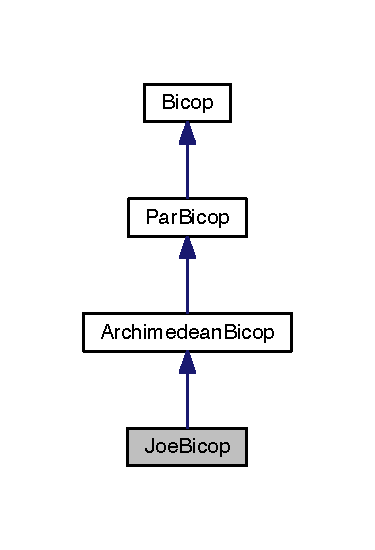
\includegraphics[width=180pt]{class_joe_bicop__inherit__graph}
\end{center}
\end{figure}


Collaboration diagram for Joe\+Bicop\+:
\nopagebreak
\begin{figure}[H]
\begin{center}
\leavevmode
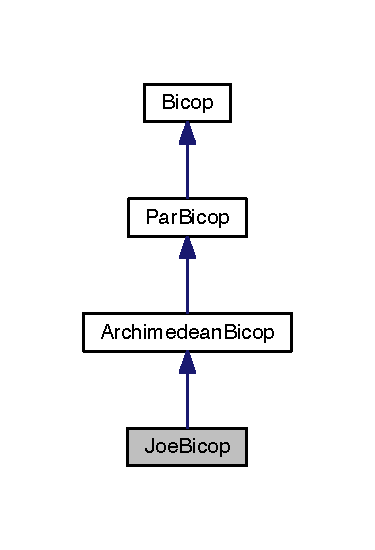
\includegraphics[width=180pt]{class_joe_bicop__coll__graph}
\end{center}
\end{figure}
\subsection*{Public Member Functions}
\begin{DoxyCompactItemize}
\item 
\mbox{\Hypertarget{class_joe_bicop_a15feadcf7028ba91c041c05f7033289d}\label{class_joe_bicop_a15feadcf7028ba91c041c05f7033289d}} 
{\bfseries Joe\+Bicop} (const Vec\+Xd \&parameters)
\item 
\mbox{\Hypertarget{class_joe_bicop_aae0e184fda31ed3a78520f70d4f4102e}\label{class_joe_bicop_aae0e184fda31ed3a78520f70d4f4102e}} 
{\bfseries Joe\+Bicop} (const Vec\+Xd \&parameters, const int \&rotation)
\item 
\mbox{\Hypertarget{class_joe_bicop_a3a9cd4684de97041f271ce1f40c32fa2}\label{class_joe_bicop_a3a9cd4684de97041f271ce1f40c32fa2}} 
Vec\+Xd {\bfseries generator} (const Vec\+Xd \&u)
\item 
\mbox{\Hypertarget{class_joe_bicop_ad4d4ff3ee52eac61b526f10a8b12c400}\label{class_joe_bicop_ad4d4ff3ee52eac61b526f10a8b12c400}} 
Vec\+Xd {\bfseries generator\+\_\+inv} (const Vec\+Xd \&u)
\item 
\mbox{\Hypertarget{class_joe_bicop_a9ee3b11b81ae825369fc1a82f922d480}\label{class_joe_bicop_a9ee3b11b81ae825369fc1a82f922d480}} 
Vec\+Xd {\bfseries generator\+\_\+derivative} (const Vec\+Xd \&u)
\item 
\mbox{\Hypertarget{class_joe_bicop_a7613e4c3cd33efac94cf2d1ee7b9869d}\label{class_joe_bicop_a7613e4c3cd33efac94cf2d1ee7b9869d}} 
Vec\+Xd {\bfseries generator\+\_\+derivative2} (const Vec\+Xd \&u)
\item 
\mbox{\Hypertarget{class_joe_bicop_a40102f50e0cd111ad75a46acdfbd80ac}\label{class_joe_bicop_a40102f50e0cd111ad75a46acdfbd80ac}} 
Vec\+Xd {\bfseries hinv} (const Mat\+Xd \&u)
\item 
\mbox{\Hypertarget{class_joe_bicop_a213002b8d12025e0aa4a3e8d648a05d1}\label{class_joe_bicop_a213002b8d12025e0aa4a3e8d648a05d1}} 
Vec\+Xd {\bfseries tau\+\_\+to\+\_\+parameters} (const double \&tau)
\item 
\mbox{\Hypertarget{class_joe_bicop_adbb7cf686a892146ea2a963e781593eb}\label{class_joe_bicop_adbb7cf686a892146ea2a963e781593eb}} 
double {\bfseries parameters\+\_\+to\+\_\+tau} (const Vec\+Xd \&par)
\end{DoxyCompactItemize}
\subsection*{Additional Inherited Members}


The documentation for this class was generated from the following files\+:\begin{DoxyCompactItemize}
\item 
/\+Users/tvatter/\+Dropbox/vinecoplib/vinecopulib/include/bicop\+\_\+joe.\+hpp\item 
/\+Users/tvatter/\+Dropbox/vinecoplib/vinecopulib/src/bicop\+\_\+joe.\+cpp\end{DoxyCompactItemize}

\hypertarget{class_normal_bicop}{\section{Normal\+Bicop Class Reference}
\label{class_normal_bicop}\index{Normal\+Bicop@{Normal\+Bicop}}
}


Inheritance diagram for Normal\+Bicop\+:
\nopagebreak
\begin{figure}[H]
\begin{center}
\leavevmode
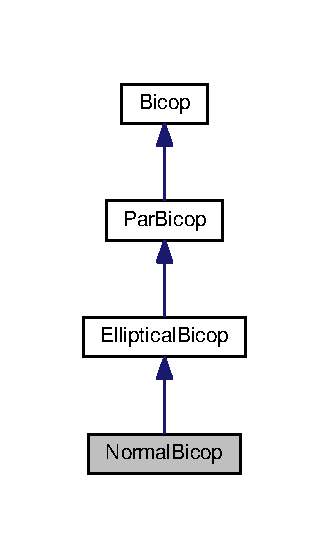
\includegraphics[width=158pt]{class_normal_bicop__inherit__graph}
\end{center}
\end{figure}


Collaboration diagram for Normal\+Bicop\+:
\nopagebreak
\begin{figure}[H]
\begin{center}
\leavevmode
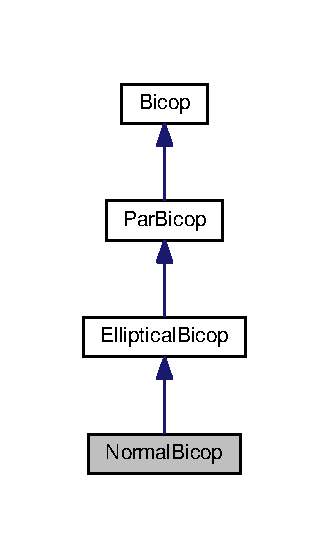
\includegraphics[width=158pt]{class_normal_bicop__coll__graph}
\end{center}
\end{figure}
\subsection*{Public Member Functions}
\begin{DoxyCompactItemize}
\item 
\hypertarget{class_normal_bicop_acc3c96fd89290fe74cc2b58a42564424}{{\bfseries Normal\+Bicop} (double rho)}\label{class_normal_bicop_acc3c96fd89290fe74cc2b58a42564424}

\item 
\hypertarget{class_normal_bicop_a2a4be0d6a8535f6a1d6eac382c89b52b}{Mat\+Xd {\bfseries get\+\_\+bounds} ()}\label{class_normal_bicop_a2a4be0d6a8535f6a1d6eac382c89b52b}

\item 
\hypertarget{class_normal_bicop_a7cb4259ed926e390e1702abd86c56abb}{Vec\+Xd {\bfseries hfunc1} (const Mat\+Xd \&u)}\label{class_normal_bicop_a7cb4259ed926e390e1702abd86c56abb}

\item 
\hypertarget{class_normal_bicop_a91b5ccb2b5d796d7d68f5ab932900403}{Vec\+Xd {\bfseries hinv1} (const Mat\+Xd \&u)}\label{class_normal_bicop_a91b5ccb2b5d796d7d68f5ab932900403}

\item 
\hypertarget{class_normal_bicop_a558c0af5dff67b781dcf4cb83222224b}{Vec\+Xd {\bfseries pdf} (const Mat\+Xd \&u)}\label{class_normal_bicop_a558c0af5dff67b781dcf4cb83222224b}

\end{DoxyCompactItemize}
\subsection*{Additional Inherited Members}


The documentation for this class was generated from the following files\+:\begin{DoxyCompactItemize}
\item 
/home/data/uni/\+Promotion/\+Cpp/vinecoplib/src/common/include/bicop\+\_\+normal.\+hpp\item 
/home/data/uni/\+Promotion/\+Cpp/vinecoplib/src/common/bicop\+\_\+normal.\+cpp\end{DoxyCompactItemize}

\hypertarget{class_par_bicop}{}\section{Par\+Bicop Class Reference}
\label{class_par_bicop}\index{Par\+Bicop@{Par\+Bicop}}


Inheritance diagram for Par\+Bicop\+:\nopagebreak
\begin{figure}[H]
\begin{center}
\leavevmode
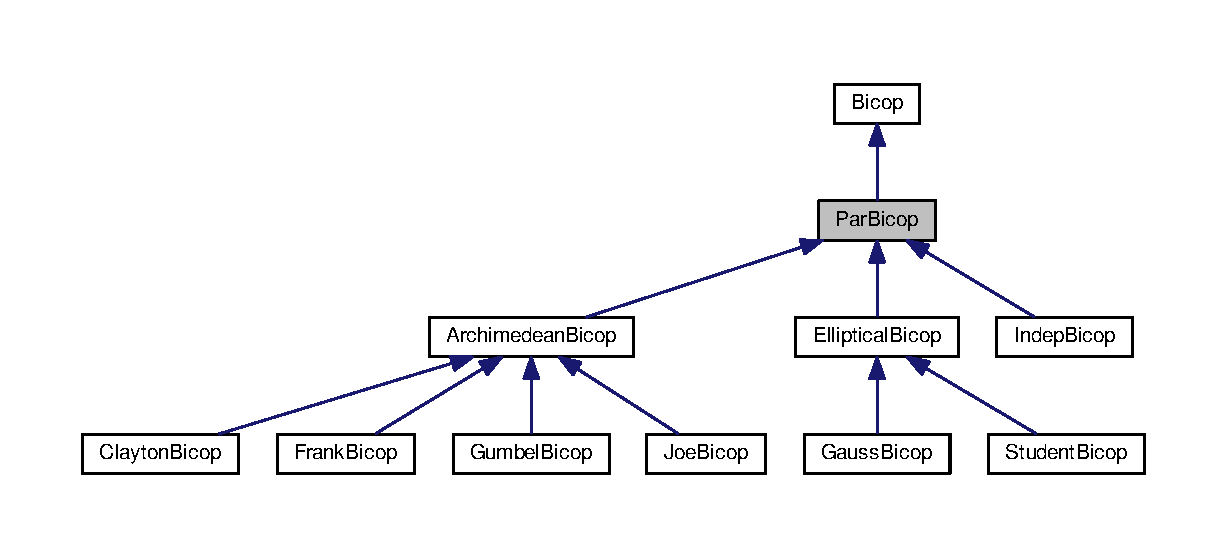
\includegraphics[width=350pt]{class_par_bicop__inherit__graph}
\end{center}
\end{figure}


Collaboration diagram for Par\+Bicop\+:\nopagebreak
\begin{figure}[H]
\begin{center}
\leavevmode
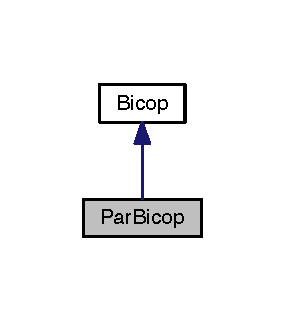
\includegraphics[width=136pt]{class_par_bicop__coll__graph}
\end{center}
\end{figure}
\subsection*{Public Member Functions}
\begin{DoxyCompactItemize}
\item 
void \hyperlink{class_par_bicop_aeab5e7031792bebc04a401a8f135d3a0}{fit} (const Mat\+Xd \&data, std\+::string method)
\item 
virtual double {\bfseries parameters\+\_\+to\+\_\+tau} (const Vec\+Xd \&parameters)=0\hypertarget{class_par_bicop_afa2abb9e5c96798e4c06e79111bb6314}{}\label{class_par_bicop_afa2abb9e5c96798e4c06e79111bb6314}

\item 
double {\bfseries calculate\+\_\+tau} ()\hypertarget{class_par_bicop_af866faf5a92ad12582b50192a033a39c}{}\label{class_par_bicop_af866faf5a92ad12582b50192a033a39c}

\item 
double \hyperlink{class_par_bicop_a190d46ae764f081e2901accade366327}{calculate\+\_\+npars} ()\hypertarget{class_par_bicop_a190d46ae764f081e2901accade366327}{}\label{class_par_bicop_a190d46ae764f081e2901accade366327}

\begin{DoxyCompactList}\small\item\em Get number of parameters. \end{DoxyCompactList}\end{DoxyCompactItemize}
\subsection*{Additional Inherited Members}


\subsection{Member Function Documentation}
\index{Par\+Bicop@{Par\+Bicop}!fit@{fit}}
\index{fit@{fit}!Par\+Bicop@{Par\+Bicop}}
\subsubsection[{\texorpdfstring{fit(const Mat\+Xd \&data, std\+::string method)}{fit(const MatXd &data, std::string method)}}]{\setlength{\rightskip}{0pt plus 5cm}void Par\+Bicop\+::fit (
\begin{DoxyParamCaption}
\item[{const Mat\+Xd \&}]{data, }
\item[{std\+::string}]{method}
\end{DoxyParamCaption}
)\hspace{0.3cm}{\ttfamily [virtual]}}\hypertarget{class_par_bicop_aeab5e7031792bebc04a401a8f135d3a0}{}\label{class_par_bicop_aeab5e7031792bebc04a401a8f135d3a0}
fitstats Fit methods and statistics


\begin{DoxyParams}{Parameters}
{\em u} & $m \times 2$ matrix of observations. \\
\hline
\end{DoxyParams}


Implements \hyperlink{class_bicop_a0ff40d8054e11ed8aaa4956c7fd84e89}{Bicop}.



The documentation for this class was generated from the following files\+:\begin{DoxyCompactItemize}
\item 
/home/n5/dev/cpp/vinecopulib/include/bicop\+\_\+parametric.\+hpp\item 
/home/n5/dev/cpp/vinecopulib/src/bicop\+\_\+parametric.\+cpp\end{DoxyCompactItemize}

\hypertarget{class_student_bicop}{}\section{Student\+Bicop Class Reference}
\label{class_student_bicop}\index{Student\+Bicop@{Student\+Bicop}}


Inheritance diagram for Student\+Bicop\+:\nopagebreak
\begin{figure}[H]
\begin{center}
\leavevmode
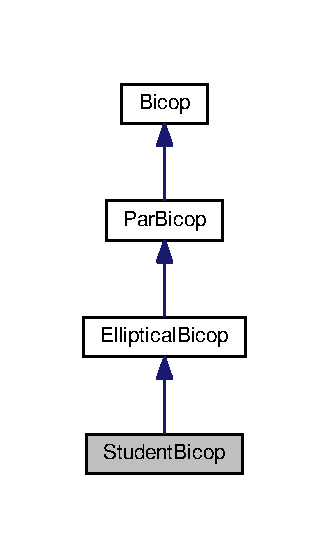
\includegraphics[width=158pt]{class_student_bicop__inherit__graph}
\end{center}
\end{figure}


Collaboration diagram for Student\+Bicop\+:\nopagebreak
\begin{figure}[H]
\begin{center}
\leavevmode
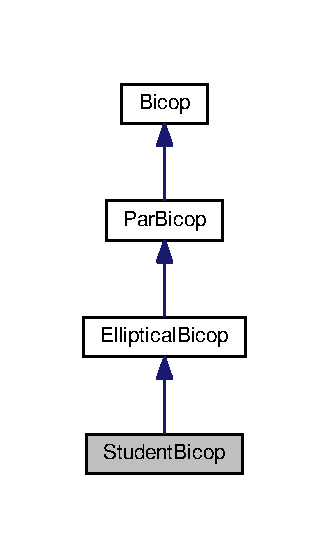
\includegraphics[width=158pt]{class_student_bicop__coll__graph}
\end{center}
\end{figure}
\subsection*{Public Member Functions}
\begin{DoxyCompactItemize}
\item 
{\bfseries Student\+Bicop} (const Vec\+Xd \&parameters)\hypertarget{class_student_bicop_a3c022a1efe1060453b3418f1fa55ebaa}{}\label{class_student_bicop_a3c022a1efe1060453b3418f1fa55ebaa}

\item 
{\bfseries Student\+Bicop} (const Vec\+Xd \&parameters, const int \&rotation)\hypertarget{class_student_bicop_a74ee1a778893916dd4fe0745562d784c}{}\label{class_student_bicop_a74ee1a778893916dd4fe0745562d784c}

\item 
Vec\+Xd {\bfseries pdf\+\_\+default} (const Mat\+Xd \&u)\hypertarget{class_student_bicop_a398dcd183989b356e63b7b929b062b39}{}\label{class_student_bicop_a398dcd183989b356e63b7b929b062b39}

\item 
Vec\+Xd {\bfseries hfunc1\+\_\+default} (const Mat\+Xd \&u)\hypertarget{class_student_bicop_ac7b273165caa154d649bb0f2e25833c6}{}\label{class_student_bicop_ac7b273165caa154d649bb0f2e25833c6}

\item 
Vec\+Xd {\bfseries hinv1\+\_\+default} (const Mat\+Xd \&u)\hypertarget{class_student_bicop_abf90b4ed51ca88f166e6ed679c22e183}{}\label{class_student_bicop_abf90b4ed51ca88f166e6ed679c22e183}

\end{DoxyCompactItemize}
\subsection*{Additional Inherited Members}


The documentation for this class was generated from the following files\+:\begin{DoxyCompactItemize}
\item 
/home/n5/dev/cpp/vinecopulib/include/bicop\+\_\+student.\+hpp\item 
/home/n5/dev/cpp/vinecopulib/src/bicop\+\_\+student.\+cpp\end{DoxyCompactItemize}

%--- End generated contents ---

% Index
\newpage
\phantomsection
\addcontentsline{toc}{chapter}{Index}
\printindex

\end{document}
